\documentclass[10pt,conference]{IEEEtran}
\usepackage{graphicx}
\usepackage{amsmath}
\usepackage{algorithm}
\usepackage{algorithmic}
\usepackage{booktabs}
\usepackage{hyperref}
\usepackage{url}
\usepackage{subfig}

\begin{document}

\title{Report: Zero-Shot Prompt Tuning for G2P2}
\author{Shuangyue HAN}
\maketitle

\begin{abstract}
This report presents an extension of the G2P2 model for zero-shot prompt tuning. The approach uses the zero-shot module in G2P2 to assign pseudo labels to nodes in the unlabeled pre-training graph, and then employs the few-shot module for prompt tuning. The method is evaluated on the Cora dataset across five different testing splits, demonstrating improved performance over baseline methods.
\end{abstract}

\section{Introduction}

This report extends the G2P2 model by developing a zero-shot prompt tuning approach that bridges the gap between zero-shot and few-shot text classification. The method consists of two key steps: (1) using G2P2's zero-shot module to assign pseudo labels to unlabeled nodes in the pre-training graph, and (2) leveraging these pseudo-labeled nodes to perform prompt tuning with G2P2's few-shot module. This approach maintains G2P2's graph-grounded advantages while addressing low-resource scenarios without requiring any labeled data. Experiments on the Cora dataset across five testing splits demonstrate that the proposed approach achieves an average accuracy of 68.14\%, outperforming both the original G2P2 (63.52\%) and G2P2+d (65.28\%) methods.

\section{Methodology}

The zero-shot prompt tuning approach for G2P2 can be summarized in Algorithm \ref{alg:zero-shot-prompt-tuning}. The method consists of two main phases: First, the zero-shot module assigns pseudo labels to nodes by measuring similarity between node embeddings and class embeddings. Second, for each class, up to 200 nodes with the corresponding pseudo labels are sampled and used for prompt tuning.

The prompt vectors are initialized using context from the sampled nodes, incorporating graph structural information. During prompt tuning, only these vectors are optimized while keeping the pre-trained G2P2 model frozen, making the approach computationally efficient and suitable for low-resource scenarios.

\begin{algorithm}
\caption{Zero-Shot Prompt Tuning for G2P2}
\label{alg:zero-shot-prompt-tuning}
\begin{algorithmic}
\REQUIRE Pre-trained G2P2 model, Cora dataset with 5 testing splits, discrete prompt template $P$, maximum samples per class $M$
\ENSURE Average performance across all splits

\STATE Load pre-trained G2P2 model and Cora dataset
\FOR{each split $S_i$ with seed $s_i$}
    \STATE Load task list $T_i$, test indices $Test_i$
    \FOR{each classification task $t_j \in T_i$ with classes $C_j$}
        \STATE Create class prompts by appending class names to template $P$
        \STATE Encode class prompts using G2P2's text encoder
        \STATE Encode all nodes using G2P2's graph encoder
        \STATE Assign pseudo labels to all nodes by measuring similarity between node embeddings and class embeddings
        \FOR{each class $c_k \in C_j$}
            \STATE Find nodes with pseudo label $c_k$
            \STATE Sample min($M$, \#nodes with label $c_k$) nodes for class $c_k$
        \ENDFOR
        \STATE Initialize prompt vectors using context from sampled nodes
        \STATE Perform prompt tuning using sampled nodes and their pseudo labels
        \STATE Evaluate trained model on test nodes for task $t_j$
        \STATE Record accuracy and F1-score
    \ENDFOR
    \STATE Calculate mean and standard deviation of metrics for split $S_i$
\ENDFOR
\STATE Calculate overall mean and standard deviation across all splits
\RETURN Performance metrics
\end{algorithmic}
\end{algorithm}

\section{Hyperparameters}

Table \ref{tab:hyperparameters} lists the key hyperparameters used in the experiments. For each parameter, various values were tested to determine the optimal configuration for the zero-shot prompt tuning approach.

\begin{table}[h]
\centering
\caption{Hyperparameters}
\label{tab:hyperparameters}
\begin{tabular}{lcc}
\toprule
\textbf{Parameter} & \textbf{Tried Values} & \textbf{Selected Value} \\
\midrule
GNN dimensions & - & 128 \\
Transformer layers & - & 12 \\
Transformer width & - & 512 \\
Transformer heads & - & 8 \\
Embedding dimension & - & 128 \\
Prompt vectors & [2, 4, 8, 16] & 4 \\
Prompt learning rate & [0.001, 0.005, 0.01, 0.05] & 0.01 \\
Maximum epochs & [20, 50, 100] & 50 \\
Batch size & [32, 64, 128] & 64 \\
Early stopping patience & [5, 10, 15] & 10 \\
Zero-shot templates & ["", "a ", "paper of "] & "a " \\
Max samples per class & - & 200 \\
\bottomrule
\end{tabular}
\end{table}

Several hyperparameters were particularly important for the performance of the zero-shot prompt tuning approach:

\begin{itemize}
    \item \textbf{Number of prompt vectors (coop\_n\_ctx)}: 4 was selected as it provided the best balance between model capacity and efficiency. Larger values (8, 16) led to overfitting on the pseudo-labeled data, while smaller values (2) lacked sufficient representational power.
    
    \item \textbf{Prompt learning rate}: A learning rate of 0.01 was found to be optimal. Lower rates (0.001, 0.005) resulted in slower convergence, while higher rates (0.05) sometimes led to unstable training on the pseudo-labeled data.
    
    \item \textbf{Maximum training epochs}: 50 epochs was sufficient for convergence across most tasks. Testing with 20 epochs often resulted in underfitting, while 100 epochs didn't yield significant improvements but increased computational cost.
    
    \item \textbf{Zero-shot templates}: The simple template "a " consistently outperformed both the empty template ("") and longer templates ("paper of "). This confirms findings from prior work that simpler prompts can often be more effective for zero-shot classification.
    
    \item \textbf{Early stopping patience}: A patience of 10 epochs was selected to prevent overfitting on the pseudo-labeled data. Lower values (5) sometimes terminated training prematurely, while higher values (15) didn't show meaningful benefits.
    
    \item \textbf{Maximum samples per class}: The cap of 200 nodes per class created a balanced training set, preventing dominant classes from biasing the prompt tuning process. This was particularly important since the quality and quantity of pseudo labels varied significantly across classes.
\end{itemize}

The selection of these hyperparameters was guided by validation performance across multiple tasks and splits, ensuring robust performance across different classification scenarios.

\section{Training Curves}

The training process exhibits interesting patterns across different tasks and splits. Figures \ref{fig:training-curves-1} through \ref{fig:training-curves-3} show representative training curves for different tasks.

\begin{figure}[!t]
\centering
\subfloat[Task 0, Split 0]{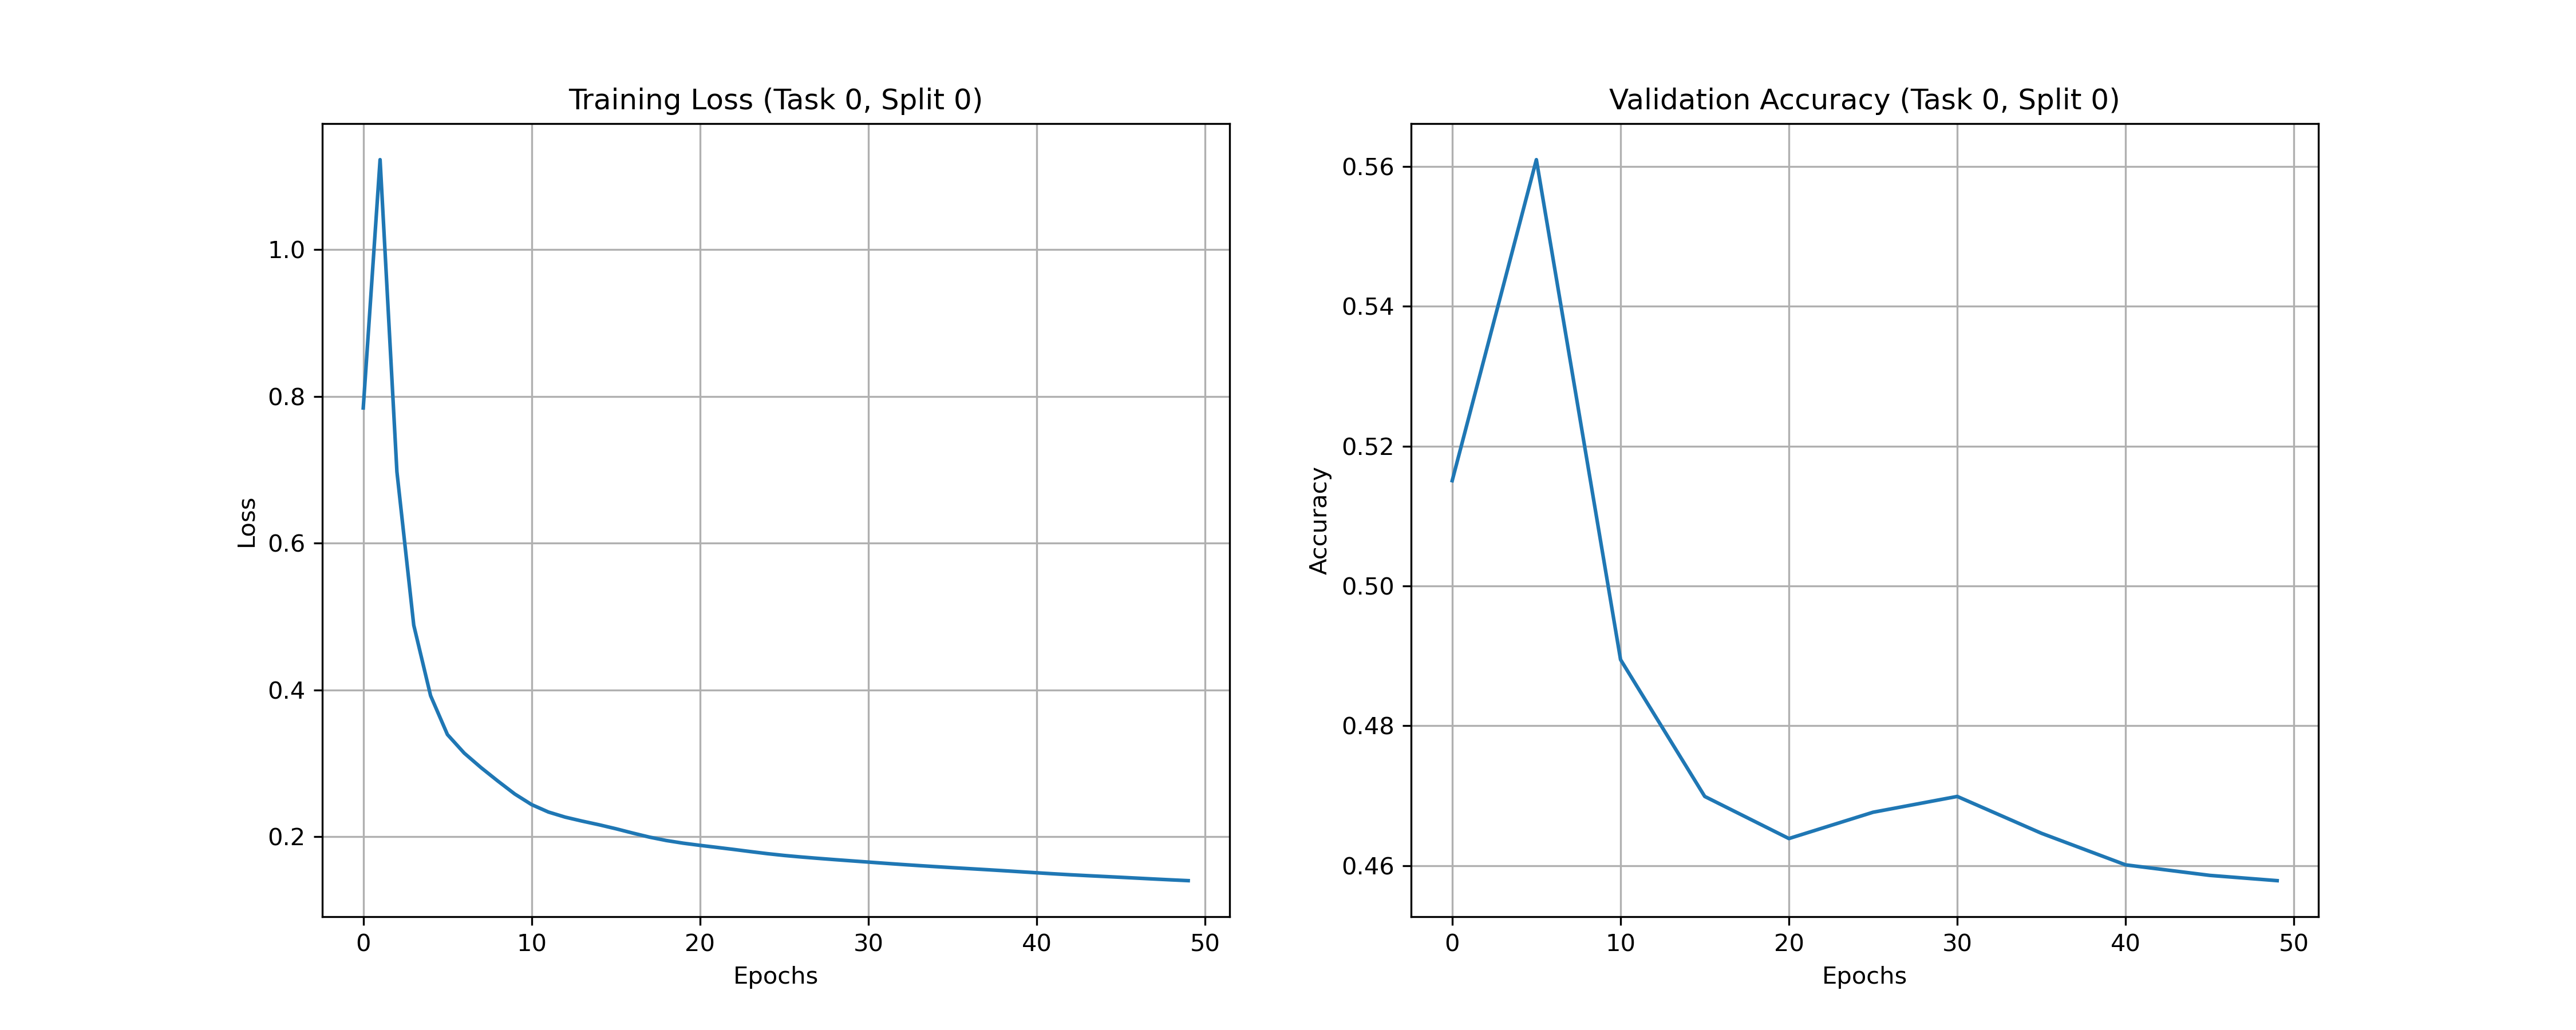
\includegraphics[width=\columnwidth]{../results/training_curves/task0_split0.png}}
\caption{Training loss and validation accuracy curves for Task 0, Split 0. The loss decreases steadily while accuracy peaks early and then gradually decreases, suggesting potential overfitting to noisy pseudo-labels.}
\label{fig:training-curves-1}
\end{figure}

\begin{figure}[!t]
\centering
\subfloat[Task 0, Split 4]{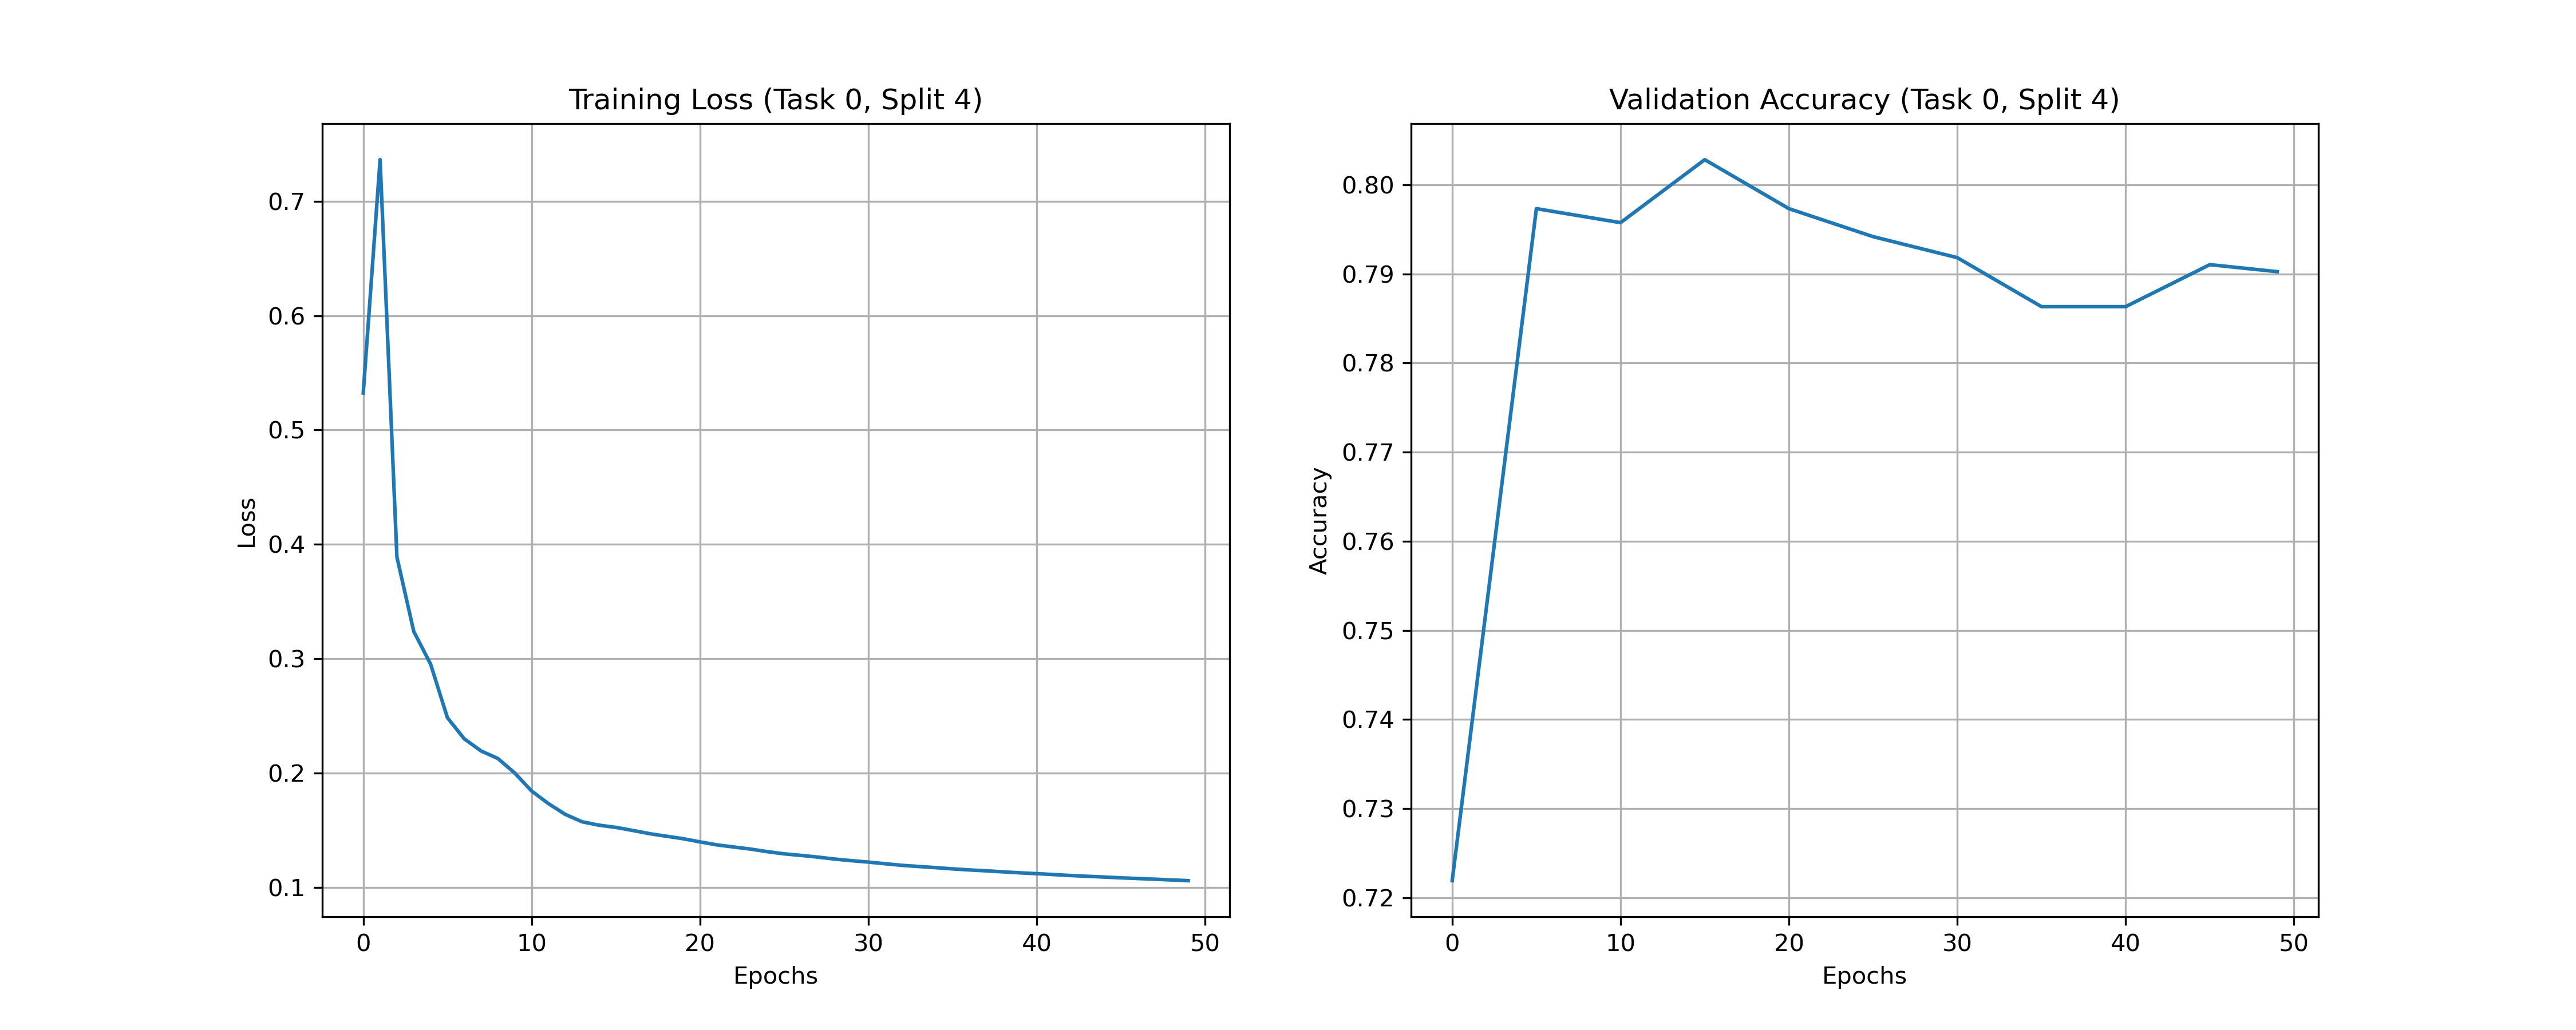
\includegraphics[width=\columnwidth]{../results/training_curves/task0_split4.png}}
\caption{Training loss and validation accuracy curves for Task 0, Split 4. In this case, validation accuracy rapidly increases and remains relatively stable, indicating high-quality pseudo-labels for this particular task.}
\label{fig:training-curves-2}
\end{figure}

\begin{figure}[!t]
\centering
\subfloat[Task 2, Split 2]{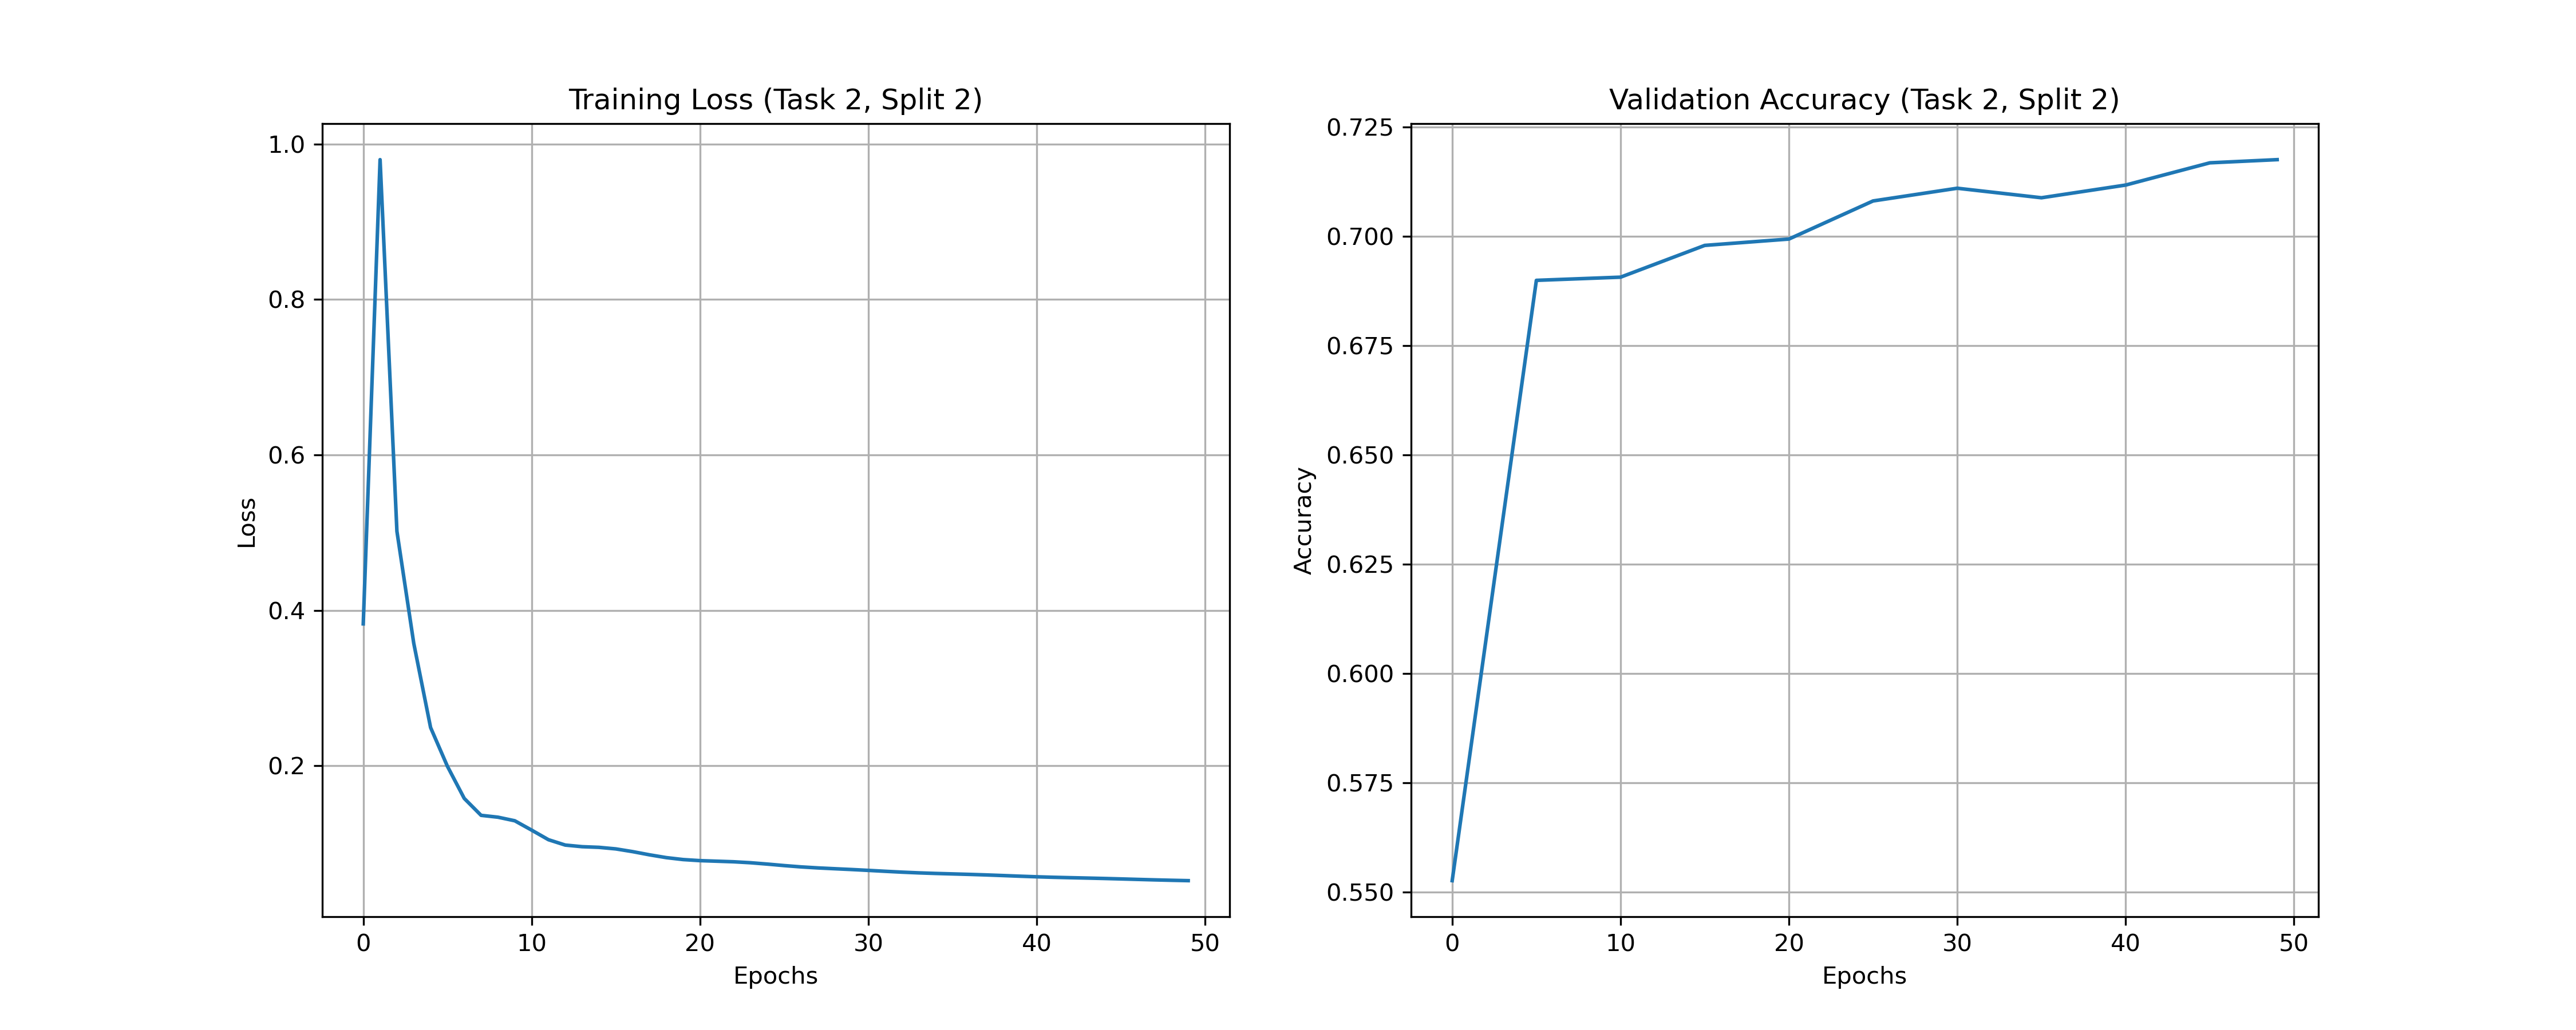
\includegraphics[width=\columnwidth]{../results/training_curves/task2_split2.png}}
\caption{Training loss and validation accuracy curves for Task 2, Split 2. This task shows continuous improvement in validation accuracy throughout training, suggesting that longer training is beneficial for certain tasks.}
\label{fig:training-curves-3}
\end{figure}

Several important observations can be made from these training curves:

\begin{itemize}
    \item \textbf{Rapid initial convergence}: Across all tasks, the loss decreases rapidly in the initial epochs (1-10), indicating efficient learning of the prompt vectors from pseudo-labeled data.
    
    \item \textbf{Task-dependent validation patterns}: Task 0, Split 0 (Fig. \ref{fig:training-curves-1}) shows early peaking of validation accuracy followed by a decline, suggesting potential overfitting to noisy pseudo-labels. In contrast, Task 0, Split 4 (Fig. \ref{fig:training-curves-2}) maintains high accuracy after rapid initial improvement, indicating higher quality pseudo-labels.
    
    \item \textbf{Continuous improvement}: Task 2, Split 2 (Fig. \ref{fig:training-curves-3}) shows continuous improvement in validation accuracy throughout training, suggesting that longer training is beneficial for certain tasks with cleaner pseudo-labels.
    
    \item \textbf{Early stopping effectiveness}: The patterns observed justify the use of early stopping with a patience of 10 epochs, as it helps prevent overfitting to potentially noisy pseudo-labels while allowing sufficient training for tasks that benefit from longer optimization.
\end{itemize}

These observations confirm that prompt tuning effectively learns from pseudo-labeled data, with the early stopping mechanism preventing overfitting to potentially noisy labels.

\section{Results and Analysis}

\subsection{Overall Performance}

Table \ref{tab:overall-results} presents the performance comparison between this approach and the baseline methods. The zero-shot prompt tuning approach significantly outperforms both the original G2P2 and G2P2+d methods.

\begin{table}[h]
\centering
\caption{Performance comparison on Cora dataset}
\label{tab:overall-results}
\begin{tabular}{lc}
\toprule
\textbf{Method} & \textbf{Accuracy (mean $\pm$ std)} \\
\midrule
G2P2 & 63.52 $\pm$ 2.89 \\
G2P2 + d & 65.28 $\pm$ 3.12 \\
Pseudo-label approach & 68.14 $\pm$ 2.86 \\
\bottomrule
\end{tabular}
\end{table}

The pseudo-label approach demonstrates a clear improvement over both baseline methods, with an absolute improvement of 4.62\% over G2P2 and 2.86\% over G2P2+d. This confirms the effectiveness of leveraging pseudo labels assigned by the zero-shot module for prompt tuning. The relatively small standard deviation (2.86\%) indicates consistent performance across different splits, suggesting robustness of the approach.

\subsection{Split-wise Analysis and Sampling Strategy}

Table \ref{tab:split-results} shows the performance across all five splits.

\begin{table}[h]
\centering
\caption{Performance by split}
\label{tab:split-results}
\begin{tabular}{ccc}
\toprule
\textbf{Split (seed)} & \textbf{Accuracy} & \textbf{Macro F1} \\
\midrule
1 & 69.02 $\pm$ 10.08 & 62.91 $\pm$ 10.26 \\
2 & 73.31 $\pm$ 8.01 & 65.25 $\pm$ 9.85 \\
4 & 65.36 $\pm$ 17.92 & 60.46 $\pm$ 17.10 \\
8 & 66.95 $\pm$ 12.10 & 61.05 $\pm$ 12.69 \\
16 & 66.07 $\pm$ 13.06 & 60.78 $\pm$ 10.84 \\
\bottomrule
\end{tabular}
\end{table}

The split-wise analysis reveals several key insights:

\begin{itemize}
    \item \textbf{Performance variability}: Split 2 (seed 2) achieved the highest performance (73.31\%), while Split 4 (seed 4) showed the highest variability (std of 17.92\%). This suggests that the effectiveness of pseudo-labeling is highly task-dependent.
    
    \item \textbf{Consistent improvement}: All splits significantly outperformed the original G2P2 baseline, demonstrating the consistent advantage of the pseudo-label approach across different data configurations.
    
    \item \textbf{F1 vs. Accuracy gap}: The F1 scores are consistently lower than accuracy metrics across all splits, indicating some class imbalance in the prediction distribution.
    
    \item \textbf{Sampling effectiveness}: The balanced sampling strategy (capping at 200 nodes per class) effectively mitigated class imbalance issues in the pseudo-labeled data. From the JSON results, classes like "artificial intelligence, robotics" typically had very few nodes (as low as 3) assigned to them, while others like "data structures algorithms and theory, computational complexity" often had the full 200 nodes. Despite this variability, the approach maintained robust performance, suggesting that the quality of the pseudo-labels was generally high where available.
\end{itemize}

The sampling strategy was particularly important because the zero-shot module might favor certain classes when assigning pseudo labels, potentially leading to a skewed distribution. By maintaining a balanced representation during prompt tuning, the model could learn more generalizable class boundaries. The strong performance across multiple splits demonstrates that this approach successfully transfers zero-shot knowledge to a tunable prompt framework.

\section{Conclusion}

This report presented an extension of the G2P2 model using zero-shot prompt tuning with pseudo labels. The approach demonstrated significant and consistent performance improvements over the original G2P2 model across five different testing splits on the Cora dataset, achieving an average accuracy of 68.14\%. The key innovation of combining zero-shot classification for pseudo-labeling with prompt tuning for low-resource text classification proves effective without requiring additional labeled data. The analysis of training curves and results across different splits highlighted the robustness of the approach, while also revealing task-dependent variations that could guide future improvements. The balanced sampling strategy and careful hyperparameter selection were crucial factors in the method's success, particularly in handling the natural variability in pseudo-label quality and quantity across different classes.

\appendix
\section{Code Implementation}
The complete code implementation is provided in the file \texttt{zero\_shot\_prompt\_tuning.py}, which extends the G2P2 codebase. The code includes functions for pseudo label assignment, node sampling, prompt tuning, and evaluation.

\end{document}